\begin{figure}[t]
\centering
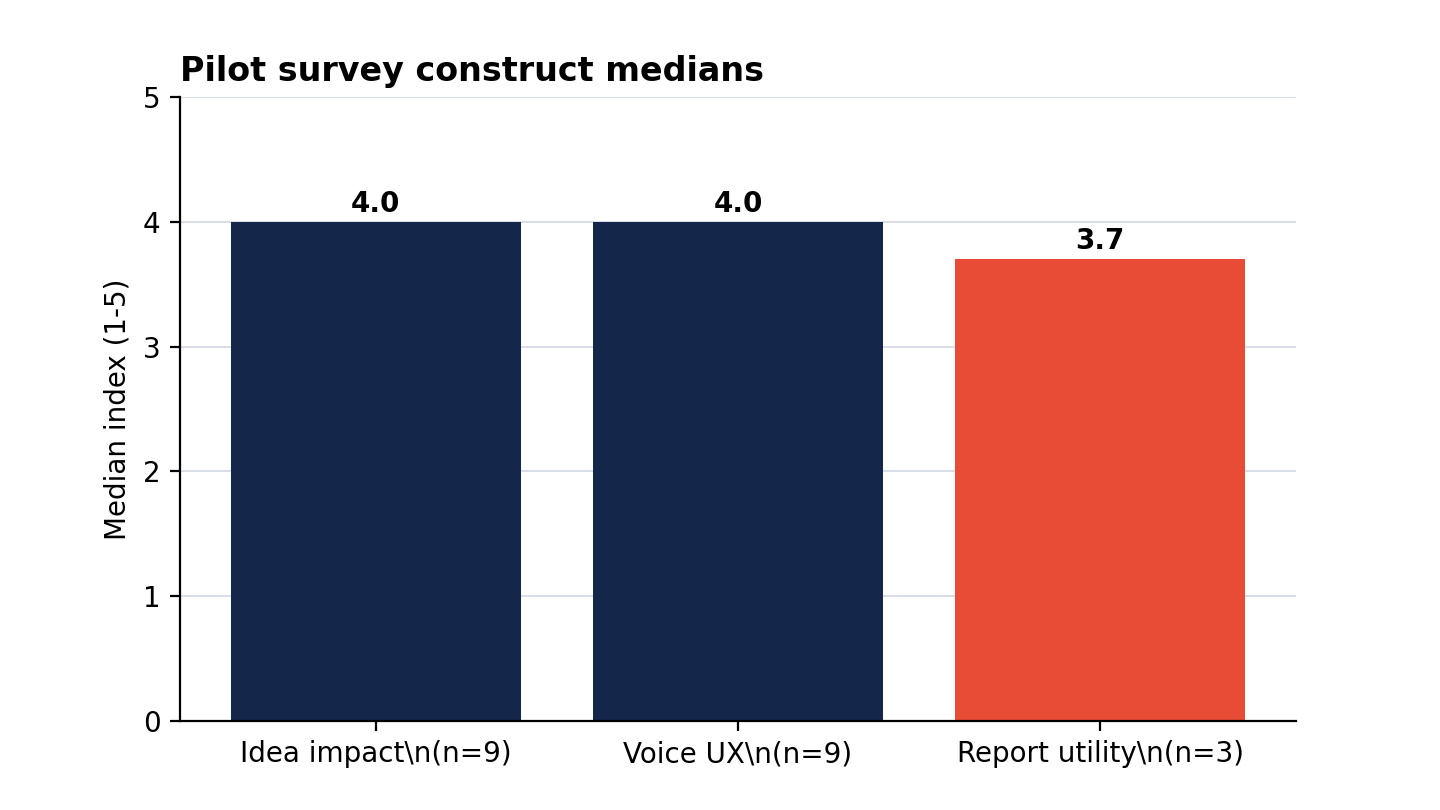
\includegraphics[width=\linewidth]{figures/pilot_survey_constructs.png}
\caption{Descriptive pilot survey construct medians. Idea impact and voice UX use all valid research feedback submissions (N=9); report utility is available only when a post-debate report was shown (n=3).}
\label{fig:pilot-survey-constructs}
\end{figure}

\begin{figure}[t]
\centering
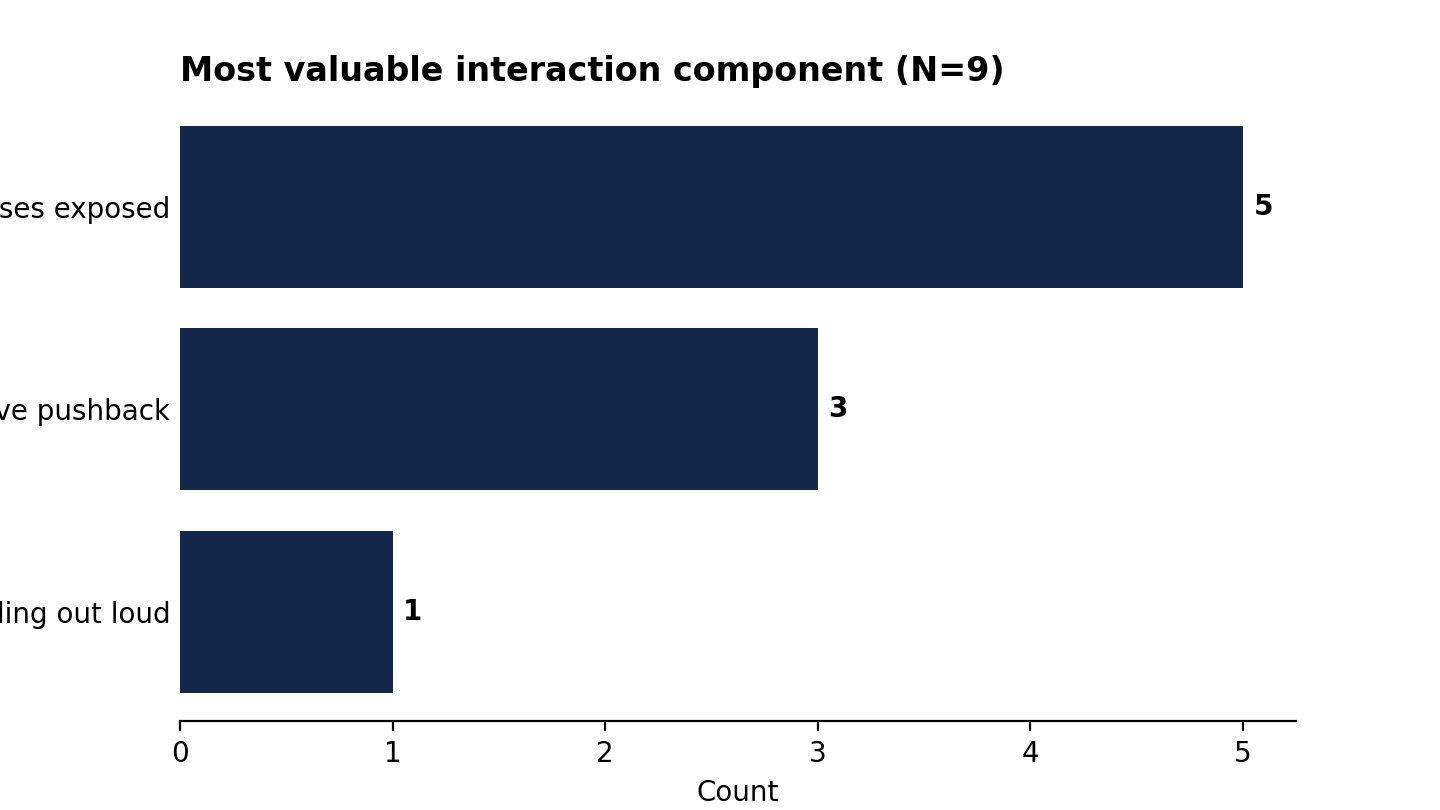
\includegraphics[width=\linewidth]{figures/most_valuable_counts.png}
\caption{Participants most often selected weakness exposure as the most valuable component of the interaction. Counts are descriptive because the formative pilot sample is small (N=9).}
\label{fig:most-valuable-counts}
\end{figure}

\begin{figure}[t]
\centering
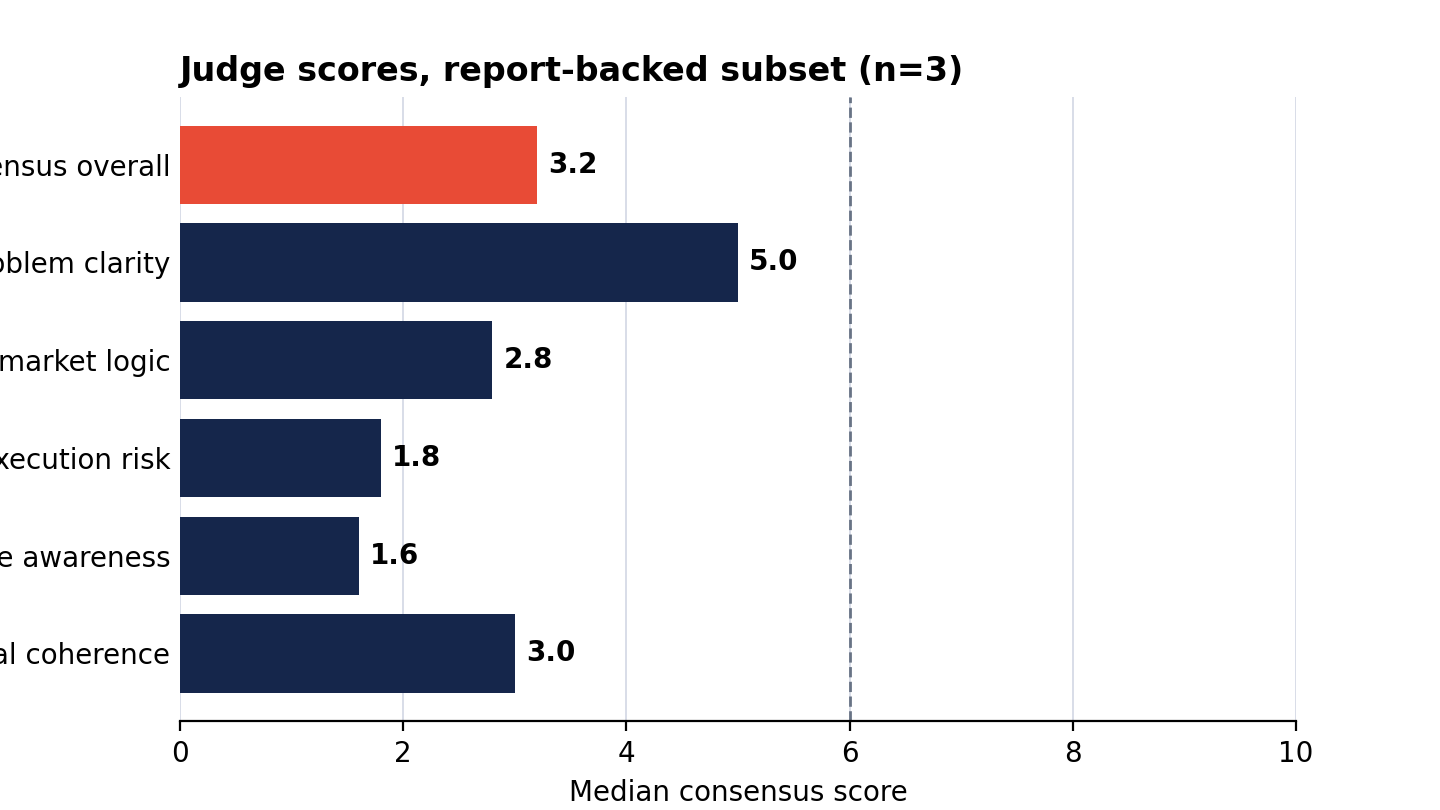
\includegraphics[width=\linewidth]{figures/judge_scores_report_subset.png}
\caption{Consensus judge scores for the report-backed subset (n=3). The dashed threshold at 6.0 indicates the founder-win cutoff used by the system; all report-backed sessions were scored below this threshold.}
\label{fig:judge-scores}
\end{figure}

\begin{table}[t]
\centering
\small
\begin{tabular}{lccc}
\toprule
Measure & n & Median & IQR \\
\midrule
Idea impact index & 9 & 4.0 & 1.8 \\
Voice UX index & 9 & 4.0 & 1.3 \\
Report utility index & 3 & 3.7 & 1.7 \\
Consensus overall score & 3 & 3.2 & 1.2 \\
\bottomrule
\end{tabular}
\caption{Descriptive outcomes from the formative pilot. Report utility and judge scores are limited to the report-backed subset.}
\label{tab:pilot-results}
\end{table}
